%%%%%%%%%%%%%%%%%%%%%%%%%%%%%%%%%%%%%%%%%%%%%%%%%%%%%%%%%%%%%%%%%%%%%%%%%%%%%%%%%%%%%%
% Modelo de relatório de Disciplina de MLP a partir da
% classe latex iiufrgs disponivel em http://github.com/schnorr/iiufrgs
%%%%%%%%%%%%%%%%%%%%%%%%%%%%%%%%%%%%%%%%%%%%%%%%%%%%%%%%%%%%%%%%%%%%%%%%%%%%%%%%%%%%%%

%%%%%%%%%%%%%%%%%%%%%%%%%%%%%%%%%%%%%%%%%%%%%%%%%%%%%%%%%%%%%%%%%%%%%%%%%%%%%%%%%%%%%%
% Definição do tipo / classe de documento e estilo usado
%%%%%%%%%%%%%%%%%%%%%%%%%%%%%%%%%%%%%%%%%%%%%%%%%%%%%%%%%%%%%%%%%%%%%%%%%%%%%%%%%%%%%%
%
\documentclass[rel_mlp]{iiufrgs}

%%%%%%%%%%%%%%%%%%%%%%%%%%%%%%%%%%%%%%%%%%%%%%%%%%%%%%%%%%%%%%%%%%%%%%%%%%%%%%%%%%%%%%
% Importação de pacotes
%%%%%%%%%%%%%%%%%%%%%%%%%%%%%%%%%%%%%%%%%%%%%%%%%%%%%%%%%%%%%%%%%%%%%%%%%%%%%%%%%%%%%%
% (a A seguir podem ser importados os pacotes necessários para o documento, de acordo 
% com a necessidade)
%
\usepackage{url}
\usepackage{hyperref}
\usepackage{verbatim}
\usepackage[brazilian]{babel}	    % para texto escrito em pt-br
\usepackage[utf8]{inputenc}         % pacote para acentuação
\usepackage{graphicx}         	    % pacote para importar figuras
\usepackage[T1]{fontenc}            % pacote para conj. de caracteres correto
\usepackage{times}                  % pacote para usar fonte Adobe Times
\usepackage{enumerate}              % para lista de itens com letras
\usepackage{breakcites}
\usepackage{titlesec}
\usepackage{enumitem}
\usepackage{titletoc}               
\usepackage{listings}			    % para listagens de código-fonte
\usepackage{mathptmx}               % p/ usar fonte Adobe Times nas formulas matematicas
\usepackage{url}                    % para formatar URLs
%\usepackage{color}				    % para imagens e outras coisas coloridas
%\usepackage{fixltx2e}              % para subscript
%\usepackage{amsmath}               % para \epsilon e matemática
%\usepackage{amsfonts}
%\usepackage{setspace}			    % para mudar espaçamento dos parágrafos
%\usepackage[table,xcdraw]{xcolor}  % para tabelas coloridas
%\usepackage{longtable}             % para tabelas compridas (mais de uma página)
%\usepackage{float}
%\usepackage{booktabs}
%\usepackage{tabularx}
%\usepackage[breaklinks]{hyperref}
\usepackage{listings}
\usepackage{xcolor} % for setting colors

% set the default code style
\lstset{
	frame=tb, % draw a frame at the top and bottom of the code block
	tabsize=4, % tab space width
	showstringspaces=false, % don't mark spaces in strings
	numbers=left, % display line numbers on the left
	commentstyle=\color{green}, % comment color
	keywordstyle=\color{blue}, % keyword color
	stringstyle=\color{red} % string color
}

\usepackage[alf,abnt-emphasize=bf]{abntex2cite}	% pacote para usar citações abnt

%%%%%%%%%%%%%%%%%%%%%%%%%%%%%%%%%%%%%%%%%%%%%%%%%%%%%%%%%%%%%%%%%%%%%%%%%%%%%%%%%%%%%%
% Macros, ajustes e definições
%%%%%%%%%%%%%%%%%%%%%%%%%%%%%%%%%%%%%%%%%%%%%%%%%%%%%%%%%%%%%%%%%%%%%%%%%%%%%%%%%%%%%%
%

% define estilo de parágrafo para citação longa direta:
\newenvironment{citacao}{
    %\singlespacing
    %\footnotesize
    \small
    \begin{list}{}{
        \setlength{\leftmargin}{4.0cm}
        \setstretch{1}
        \setlength{\topsep}{1.2cm}
        \setlength{\listparindent}{\parindent}
    }
    \item[]}{\end{list}
}

% adiciona a fonte em figuras e tabelas
\newcommand{\fonte}[1]{\\Fonte: {#1}}

% Ative o seguinte caso alguma nota de rodapé fique muito longa e quebre entre múltiplas
% páginas
%\interfootnotelinepenalty=10000

%%%%%%%%%%%%%%%%%%%%%%%%%%%%%%%%%%%%%%%%%%%%%%%%%%%%%%%%%%%%%%%%%%%%%%%%%%%%%%%%%%%%%%
% Informações gerais                                   
%%%%%%%%%%%%%%%%%%%%%%%%%%%%%%%%%%%%%%%%%%%%%%%%%%%%%%%%%%%%%%%%%%%%%%%%%%%%%%%%%%%%%%

% título
\title{Jogo Pedagógico em C++} 

% autor
\author{Dalcin}{Leonardo} % {sobrenome}{nome}
\author{Ramos da Rosa}{Paulo Ricardo} 
\author{Degrazia}{Pietro} 
%\author{Autor2}{Aluno} % {sobrenome}{nome} 1 para cada aluno

% Professor orientador da disciplina
\advisor[Prof.~Dr.]{Mello Schnorr}{Lucas}

% Nome do(s) curso(s):
\course{Curso de Graduação em Ciência da Computa{\c{c}}{\~a}o e Engenharia de Computação}

% local da realização do trabalho 
\location{Porto Alegre}{RS} 

% data da entrega do trabalho (mês e ano)
\date{12}{2018}


% Palavras chave
\keyword{Palavra-chave1}
\keyword{Palavra-chave2}
\keyword{Palavra-chave3}


%%%%%%%%%%%%%%%%%%%%%%%%%%%%%%%%%%%%%%%%%%%%%%%%%%%%%%%%%%%%%%%%%%%%%%%%%%%%%%%%%%%%%%
% Início do documento e elementos pré-textuais
%%%%%%%%%%%%%%%%%%%%%%%%%%%%%%%%%%%%%%%%%%%%%%%%%%%%%%%%%%%%%%%%%%%%%%%%%%%%%%%%%%%%%%

% Declara início do documento
\begin{document}

% inclui folha de rosto 
\maketitle      

\selectlanguage{brazilian}

% Sumario
\tableofcontents



%%%%%%%%%%%%%%%%%%%%%%%%%%%%%%%%%%%%%%%%%%%%%%%%%%%%%%%%%%%%%%%%%%%%%%%%%%%%%%%%%%%%%
% Aqui comeca o texto propriamente dito
%%%%%%%%%%%%%%%%%%%%%%%%%%%%%%%%%%%%%%%%%%%%%%%%%%%%%%%%%%%%%%%%%%%%%%%%%%%%%%%%%%%%%

%espaçamento entre parágrafos
%\setlength{\parskip}{6 pt}

\selectlanguage{brazilian}



%%%%%%%%%%%%%%%%%%%%%%%%%%%%%%%%%%%%%%%%%%%%%%%%%%%%%%%%%%%%%%%%%%%%%%%%%%%%%%%%%%%%%
% Introdução
%
\chapter{Introdução} \label{intro}

%Este capítulo tem o objetivo de descrever os detalhes necessários à correta formatação do documento. As informações aqui apresentadas devem ser suficientes para formatar corretamente o documento no ambiente \LaTeX.

%Os \textbf{Capítulos} são sempre iniciados com o comando \texttt{\char'134chapter}, que coloca-os em uma nova folha, em letras maiúsculas, numerados e  alinhados à esquerda. Para os \textbf{capítulos não-numerados} (Listas, Resumo, Abstract, Referências, etc.), o título é centralizado na linha Para tanto, usar o comando \texttt{\char'134chapter*}. Para ambos, são deixados 90 pt de espaçamento anterior (ou seja, distância da margem superior) e 42 pt de espaçamento posterior (espaço até o início do texto ou primeira subdivisão). 

%Todos os \textbf{demais parágrafos de texto} são escritos em espaçamento simples, com observância de 6 pt de espaçamento em relação ao parágrafo seguinte. O estilo atual já considera essas retrições. 

Este trabalho tem como objetivo a implementação em C++ de um jogo pedagógico que visa ensinar diversos conceitos da cadeira de Modelos de Linguagens de Programação em diferentes níveis de profundidade. O programa permitirá que o usuário compartilhe seus resultados e confira respostas de outros colegas, assim como explicações e links para referências sobre o assunto.

\section{Projeto}

%As demais subdivisões do texto (seções, subseções, etc.) são formatadas com o título alinhado sempre à esquerda, precedido da respectiva numeração. Para tanto, no \LaTeX, você deve utilizar os comandos \texttt{\char'134section},  \texttt{\char'134subsection} e  \texttt{\char'134subsubsection}.

%São permitidas subdivisões até o 5º nível (onde o capítulo é o 1º. nível), porém no sumário inclui-se somente os títulos até o nível 3\footnote{O formato adotado pela ABNT prevê apenas três níveis (capítulo, seção e subseção).}. Assim, \texttt{\char'134subsubsection} não é aconselhado. 

A proposta do projeto consta em, dada uma linguagem de programação escolhida pelo grupo dentre as pré-selecionadas pelo professor, desenvolver uma aplicação com duas implementações: uma puramente orientada a objetos e outra puramente funcional, contendo alguma forma de paralelismo. C++17 será a linguagem utilizada para ambas as versões.

\section{Sobre o jogo}
O projeto será um jogo de perguntas e respostas sobre a disciplina de Modelos de Linguagem de Programação, aos moldes dos programas "Show do Milhão" e "Quem quer ser um milionário?", com a objetivo de ajudar o estudante na disciplina. O jogo contará com explicações sobre o conteúdo das perguntas e poderá ser feito a consulta das respostas dos outros jogadores. 

\chapter{C++17}\label{c++}

\section{Origem}
A linguagem C++ foi introduzida inicialmente em 1985 por Bjarne Stroustrup, herdando as características da linguagem C mas adicionando o conceito de Orientação a Objetos. Desde então, passou por diversas atualizações, estando hoje padronizada na versão ISO/IEC 14882:2017, informalmente conhecida como C++17.

\section{Programa}
Programas em C++ podem conter valores, objetos, referências, funções, enumeradores, tipos, membros de classes, templates, especializações de template e namespaces. Essas entidades são criadas através de declarações, que associam a entidade com um nome e define suas propriedades. A declaração que define todas as propriedades para usar uma entidade é chamada de definição.

Nomes encontrados em um programa são associados com a declaração em que aparecem. Eles somente são válidos no escopo em que foram declarados. Alguns nomes, dependendo da linkagem, podem referênciar entidades que aparecem em um escopo diferente.

\section{Objetos}
Programas em C++ criam, destroem, referenciam, acessam e manipulam objetos. Um objeto em C++ é uma região de armazenamento que possui:
\begin{itemize}
	\item tamanho(sizeof);
	\item requisito de alinhamento(alignof);
	\item duração de alocação(automática, estática, dinâmica, local);
	\item duração de vida(baseada na alocação ou temporária);
	\item tipo;
	\item valor(pode ser indeterminado);
	\item nome(opcional).
\end{itemize}

Objetos são criados com definições, expressões new, expressões throw, por manipulação de membros de uma union e onde objetos temporários são necessários.

\section{Classes}
Classes e estruturas são tipos definidos pelo usuário, usando especificadores de classe, que devem aparecer na sequencia a seguir.

\begin{itemize}
	\item Chave de classe - pode ser class ou struct, a única diferença entre elas é o acesso padrão, para estruturas é acesso a membro, e para classes é a membro da classe base.
	\item Atributos - sequencia opcional de atributos, noreturn, por exemplo. Também pode ser incluido especificadores de alinhamento.
	\item Nome - o identificador da classe. Opcionalmente acompanhado da palavra chave final. Caso o nome seja omitido, a classe é considerada anônima e não pode ser final.
	\item Classes base -  lista opcional de classes pai e o modelo de herança que será usado para cada uma delas.
	\item Membros - lista de membros, especificadores de acesso, declaração e definição de funções de instância, tipos e classes aninhados.
\end{itemize}

\section{Classes Abstratas}
Classes abstratas são tipos que não podem ser instanciados, mas podem ser usados como classe base. Para criar uma, basta usar o especificador virtual. Classes como essas são usadas para representar conceitos gerais, por exemplo, Forma ou Animal, esses tipos serão usados como classe base para tipos concretos como Círculo ou Cachorro. 

Não é possível usar tipos abstratos em parâmetros, tipos de retorno ou conversões. É possível usar esses tipos com ponteiros e referências.

Classes abstratas em C++ são implementadas declarando pelo menos um de seus métodos como virtual puro. Um método virtual puro é especificado colocando "=0" na sua declaração. O propósito de uma classe abstrata é prover uma base na qual outras classes podem herdar atributos e métodos. Se uma subclasse X herda de uma classe abstrata Y, ela precisa implementar todos os métodos virtuais puros, caso contrário ela será considerada uma classe abstrata também. Se ela foi instanciada, um erro de compilação ocorrerá.

\section{Polimorfismo}
Objetos de uma classe que declaram ou herdam pelo menos uma função virtual são considerados polimórficos. Dentro de cada objeto deste tipo, a implementação contém informações adicionais que são usadas por chamadas de funções virtuais e por métodos auxiliares como dynamic cast ou typeid.
\subsection{Polimorfismo por Inclusão}
Também chamado de polimorfismo de subtipo ou polimorfismo em tempo de execução, acontece durante a execução através de uma tabela virtual. O compilador não localiza o endereço da função a ser chamada em tempo de compilação, em vez disso quando o programa é executado, a função é referenciada por um ponteiro na tabela virtual.
\subsection{Polimorfismo Paramétrico}
Polimorfismo paramétrico possibilita executar um mesmo código para qualquer tipo. Em C++ polimorfismo paramétrico é implementado via templates.
Um exemplo de template utilizado no projeto é o método \textbf{max} :

	\begin{lstlisting}[language=C++, caption={Método genérico para calcular o máximo entre dois argumentos genéricos}]

#include <iostream>
#include <string>

template <class T>
T max(T a, T b) {
	return a > b ? a : b;
}

int main() {
	std::cout << ::max(9, 5) << std::endl;     // 9
	
	std::string foo("foo"), bar("bar");
	std::cout << ::max(foo, bar) << std::endl; // "foo"
}

\end{lstlisting}

Contudo, esse método não funciona em ponteiros porque comparar ponteiros é comparar o local de memória e não o conteúdo. Para funcionar com ponteiros, deve-se especificar um template para ponteiros, o que deixaria de ser polimorfismo paramétrico e passaria a ser ad-hoc.
Polimorfismo paramétrico também é chamado de polimorfismo em tempo de compilação, já que ocorre durante a compilação.


\section{Memória}
C++ possui 4 tipos de gerenciamento de memória:
\begin{itemize}
	\item Armazenamento de duração estática: são criados antes da chamada main() (salvo exceções) e destruídos na ordem reversa de criação após a saída de main().
	\item Armazenamento de duração de thread: Similar ao armazenamento estático, porém o objeto é criado com a thread e destruído com o join da thread.
	\item Armazenamento automático: Variáveis automáticas são criadas no ponto de declaração e destruídas na ordem reversa de criação de seu escopo. São alocadas automaticamente na pilha.
	\item Armazenamento dinâmico: São criadas com uma chamada new e destruídas com uma chamada delete.
\end{itemize}

\chapter{Implementação}\label{imp}
\section{Orientação a Objetos}
A implementação inicial inclui duas classes bases:
\begin{itemize}
	\item Player: Classe que será utilizada para criar informações sobre o jogador, como nome e pontuação.
	\subitem Atributos: std::string name, int score.
	\subitem Métodos: Construtor, getScore, setScore(int score).
	\item Question: Classe que conterá uma pergunta com suas alternativas e resposta.
	\subitem Atributos: std::string enunciation, std::string alternatives[4], int answer.
	\subitem Métodos: Construtor, showQuestion(): mostra a pergunta e as alternativas, respond(int alternative): recebe a resposta do usuário, askQuestion(): realiza a pergunta com os métodos showQuestion() e respond(int alternative).
\end{itemize}
Além dessas classes, uma classe Database está incluída para gravar dados do programa, essencialmente as perguntas, e uma classe Main para execução do programa.



\section{Recursos utilizados para a implementação OO}
\begin{itemize}
	\item Recursos mínimos sugeridos
	\subitem 1. Especificar e utilizar classes (utilitárias ou para representar as estruturas de dados utilizadas pelo programa).
	\begin{lstlisting}[language=C++, caption={Exemplo de classe utilizada no programa}]
	#include <iostream>
	#include <string>
	
	class Player
	{
	private:
	std::string name;
	int score;
	public:
	Player(std::string name){
	this->name = name;
	}
	int getScore()
	{
	return this->score;
	}
	void setScore(int score)
	{
	this->score = score;
	}
	};
	\end{lstlisting}
	
	\subitem 2. Fazer uso de encapsulamento e proteção dos atributos, com os devidos métodos de manipulação (setters/getters) ou propriedades de acesso, em especial com validação dos valores (parâmetros) para que estejam dentro do esperado ou gerem exceções caso contrário.
	
	Observando o Listing 3.1 o atributo  \textbf{score} é protegido pelos métodos \textbf{getScore} e \textbf{setScore}, impossibilitando algum desenvolvedor de ter acesso direto à esta propriedade do objeto \textbf{Player}. Isso centraliza a leitura e a escrita desse atributo, resultando em uma melhor organização do código.
	
	Além disso, seções do programa que precisam de entrada de dados do usuário estão devidamente protegidas contra dados indevidos, especificamente na entrada da resposta quando um laço \textit{while} impede dados inválidos. Caso a entrada não seja \textbf{int}, ela é limpa e ignorada.
	
	\begin{lstlisting}[language=C++, caption={Proteção de dados inválidos}]
	while ( !(std::cin >> answer)) {
	std::cin.clear();
	std::cin.ignore(std::numeric_limits<std::streamsize>::max(), '\n');
	std::cout << "Valor invalido\n";
	}
	\end{lstlisting}
	
	\subitem 3. Especificação e uso de construtores-padrão para a inicialização dos atributos e, sempre que possível, de construtores alternativos.
	
	O listing 3.1 também demonstra o uso de um construtor não padrão que necessita somente do atributo \textbf{name} que tem especificação de tipo, garantindo então a tipagem correta deste parametro.
	
	\subitem 4. Especificação e uso de destrutores (ou métodos de finalização), quando necessário.
	Destrutores foram especificados para mostrar uma mensagem caso sejam chamados.
	\begin{lstlisting}[language=C++, caption={Exemplo de destrutor}]
	Player::~Player()
	{
	std::cout << "Jogador deletado" << std::endl;
	}
	\end{lstlisting}
	
	\subitem 5. Organizar o código em espaços de nome diferenciados, conforme a função ou estrutura de cada classe ou módulo de programa.
	
	As classes estão separadas em arquivos .h e .cpp, para cada classe ter seu determinado espaço de nome.
	
	\begin{lstlisting}[language=C++, caption={Separação entre definição e implementação}]
	//Player.h
	#ifndef MLPQUIZAPP_PLAYER_H
	#define MLPQUIZAPP_PLAYER_H
	
	#include "Person.h"
	#include <iostream>
	#include <string>
	class Player:public Person
	{
	private:
	int _score;
	public:
	Player(std::string name);
	~Player();
	int getScore()const;
	void setScore(int score);
	void print();
	};
	
	#endif //MLPQUIZAPP_PLAYER_H
	
	//Player.cpp
	#include "Player.h"
	#include <iostream>
	#include <string>
	
	
	Player::Player(std::string name):Person(name) {
	this->_score = 0;
	}
	
	Player::~Player()
	{
	std::cout << "Jogador deletado" << std::endl;
	}
	
	void Player::setScore(int score) {
	if (score < 0) { return; }
	this->_score = score;
	}
	
	void Player::print() {
	std::cout<< "Meu nome e "<< this->getName() << " e minha pontuacao e " << this->getScore() << std::endl;
	}
	int Player::getScore() const
	{
	return _score;
	}
	\end{lstlisting}
	
	\subitem 6. Usar mecanismo de herança, em especial com a especificação de pelo menos três níveis de hierarquia, sendo pelo menos um deles correspondente a uma classe abstrata, mais genérica, a ser implementada nas classes-filhas.
	
	O projeto possui uma classe topo chamada \textbf{Object}, da qual todas as outras classes são derivadas. Ela possui um método \textbf{print} a ser sobrescrito pelas subclasses, funcionando de maneira similar ao \textit{toString} do Java. A classe abstrata \textbf{Person} é subclasse de Object e possui um atributo \textbf{name}, bem como uma implementação própria de \textbf{print}. A classe \textbf{Player} é subclasse de \textbf{Person}, herdando o atributo \textbf{name} e além de sobrescrever o método \textbf{print}, possui o atributo \textbf{score}, referente a pontuação do jogo. 
	
	\begin{figure}[h!]
		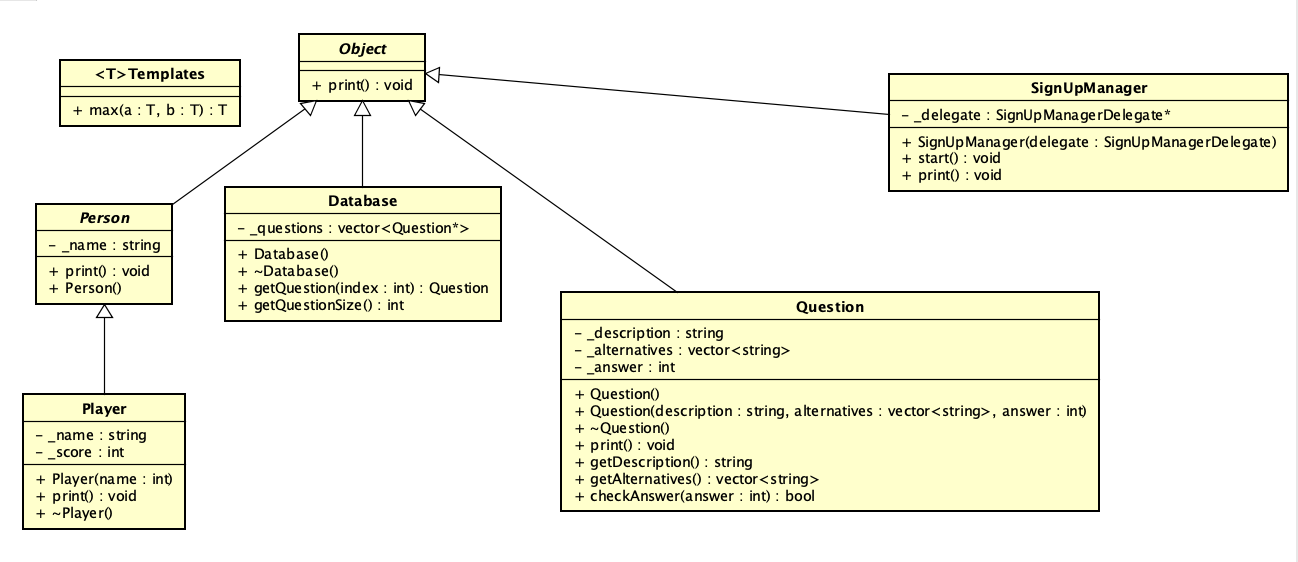
\includegraphics[width=\linewidth]{dc.png}
		\caption{Diagrama de Classes}
		\label{fig:dc}
	\end{figure}
	
	\subitem 7. Utilizar polimorfismo por inclusão (variável ou coleção genérica manipulando entidades de classes filhas, chamando métodos ou funções específicas correspondentes)
	
	O método \textbf{print} presente em todas as classes que herdam de \textbf{Object} é um exemplo de polimorfismo por inclusão, já que a classe \textbf{Person} possui uma implementação e \textbf{Player} possui outra.
	
	\begin{lstlisting}[language=C++, caption={Exemplo de polimorfismo por inclusão}]
	//Classe Person
	#include "Person.h"
	
	std::string Person::getName()
	{
	return _name;
	}
	
	Person::Person(std::string name)
	{
	this->_name = name;
	
	}
	
	void Person::print()
	{
	std::cout<< "Meu nome e "<< this->_name << std::endl;
	}
	
	//Classe Player
	#include "Player.h"
	#include <iostream>
	#include <string>
	
	
	Player::Player(std::string name):Person(name) {
	this->_score = 0;
	}
	
	Player::~Player()
	{
	std::cout << "Jogador deletado" << std::endl;
	}
	
	void Player::setScore(int score) {
	if (score < 0) { return; }
	this->_score = score;
	}
	
	void Player::print() {
	std::cout<< "Meu nome e "<< this->getName() <<
	 " e minha pontuacao e " << this->getScore() << std::endl;
	}
	int Player::getScore() const
	{
	return _score;
	}
	
	\end{lstlisting}
	
	\subitem 8. Usar polimorfismo paramétrico
	através da especificação de \textit{algoritmo} (método ou função genérico) utilizando o recurso oferecido pela linguagem (i.e., generics, templates ou similar)
	e da especificação de \textit{estrutura de dados} genérica utilizando o recurso oferecido pela linguagem.
	
	A classe \textbf{Templates} é uma classe genérica com o método \textbf{max} para calcular o máximo entre dois valores genéricos.
	
	\begin{lstlisting}[language=C++, caption={Polimorfismo paramétrico}]
	template <class T>
	T max(T a, T b) {
	return a > b ? a : b;
	}
	\end{lstlisting}
	
	\subitem 9. Usar polimorfismo por sobrecarga (vale construtores alternativos).
	
	A classe \textbf{Question} possui dois construtores: Um padrão sem argumentos, para construir uma pergunta genérica e outro com os parâmetros de enunciado, alternativas e resposta.
	
	\begin{lstlisting}[language=C++, caption={Construtores da classe Question}]
	Question::Question() {
	this->_description = "Description";
	this->_answer = 0;
	
	std::vector<std::string> alternatives {"Option 1", "Option 2"};
	this->_alternatives = alternatives;
	};
	
	Question::Question(std::string description, std::vector<std::string> alternatives, int answer) {
	this->_description = description;
	this->_alternatives = alternatives;
	this->_answer = answer;
	}
	\end{lstlisting}
	
	\subitem 10. Especificar e usar delegates.
	
	Delegates são utilizados na classe \textbf{SignUpManager} para cadastrar um jogador com o \textbf{SignUpManagerDelegate}:
	
	\begin{lstlisting}[language=C++, caption={Uso de delegate}]
	typedef void SignUpManagerDelegate(Player);
	
	class SignUpManager:Object {
	public:
	SignUpManager(SignUpManagerDelegate delegate);
	void start();
	void print();
	private:
	SignUpManagerDelegate* _delegate;
	};
	
	SignUpManager::SignUpManager(SignUpManagerDelegate delegate) {
	this->_delegate = delegate;
	};
	
	void SignUpManager::start() {
	std::string name;
	std::cout << "Escolha um nome de usuario: ";
	std::getline(std::cin, name);
	
	auto player = Player(name);
	this->_delegate(player);
	}
	\end{lstlisting}
	
	
	\item Recursos de processamento paralelo
	
	\begin{lstlisting}[language=C++, caption={Uso de Paralelismo}]
	std::vector<Question*> scrambledQuestions;
	#pragma omp parallel for
	for (int i = 0; i < _questions.size(); i++) {
	#pragma omp critical
	scrambledQuestions.push_back(_questions[i]);
	}
	\end{lstlisting}
	
	\subitem 1. Definição, uso e gerência de unidades (threads, módulos, classes, métodos, funções, trechos ou instruções) de execução concorrente e o seu sincronismo
	
	Usou-se paralelismo na função que embaralha as questões do database com o uso da biblioteca OpenMP.
	
	\subitem 2. Definição, uso e gerência de regiões críticas (variáveis, arrays, coleções ou similares)

	A seção crítica é o vetor que está sendo acessado no loop.
\end{itemize}

\section{Funcional}

\section{Recursos utilizados para a implementação Funcional}
\begin{itemize}
	\item Recursos mínimos sugeridos
	
	\subitem 1. Priorizar o uso de elementos imutáveis e funções puras (por exemplo, sempre precisar manipular listas, criar uma nova e não modificar a original, seja por recursão ou através de funções de ordem maior). TODO
	
	\subitem 2. Especificar e usar funções não nomeadas (ou lambda) TODO.
	
	\subitem 3. Especificar e usar funções que usem currying TODO.
	
	\subitem 4. Especificar funções que utilizem pattern matching ao máximo, na sua definição TODO.
	
	\subitem 5. Especificar e usar funções de ordem superior (maior) criadas pelo programador TODO.
	
	\subitem 6. Usar funções de ordem maior prontas (p.ex., map, reduce, foldr/foldl ou similares) TODO.
	
	\subitem 7. Especificar e usar funções como elementos de 1ª ordem TODO.
	
	\subitem 8.Usar recursão como mecanismo de iteração (pelo menos em funções de ordem superior que manipulem listas) TODO.
	
	\item Recursos extras
	\subitem Exemplo de recurso extra
	
	\item Recursos de processamento paralelo
		\subitem 1. Definição, uso e gerência de unidades (threads, módulos, classes, métodos, funções, trechos ou instruções) de execução concorrente e o seu sincronismo TODO
		\subitem 2. Definição, uso e gerência de regiões críticas (variáveis, arrays, coleções ou similares) TODO
	
\end{itemize}
\section{Análise da Linguagem}
Uma análise da linguagem foi feita considerando diversos aspectos, como usabilidade, simplicidade, tipos de dados, entre outros (notas de um a dez, sendo dez excelente e um péssimo).
\begin{table}[!h]
	\begin{tabular}{|l|l|l|}
		\hline
		\textbf{Critério} & \textbf{Nota} & \textbf{Avaliação} \\ \hline
		Simplicidade & 5 & \begin{tabular}[c]{@{}l@{}}Não é uma linguagem trivial de aprender, \\ já que possui muitas ferramentas\\  e  especialmente na parte funcional, é de \\ nível difícil\end{tabular} \\ \hline
		Ortogonalidade & 6 & \begin{tabular}[c]{@{}l@{}}Possui as primitivas básicas de uma\\  linguagem, como int, float, char, long.\\  Diferente de C, possui bool e string.\end{tabular} \\ \hline
		Estrutura de controle & 7 & \begin{tabular}[c]{@{}l@{}}Possui operadores básicos de controle,\\  como iteradores e variáveis\\ de controle\end{tabular} \\ \hline
		Tipos de dados & 7 & \begin{tabular}[c]{@{}l@{}}Possui suporte a classes customizadas, \\ podendo criar um tipo específico\\ ou um tipo genérico, mas algumas \\ funcionalidades não são reutilizáveis\\ por padrão, como imprimir um objeto,\\  sendo necessário reimplementar\\ o operador \textless{}\textless{}\end{tabular} \\ \hline
		Estruturas de dados & 8 & \begin{tabular}[c]{@{}l@{}}Possui estruturas de dados robustas, \\ incluindo certas bibliotecas\end{tabular} \\ \hline
		Suporte a abstração de dados & 7 & \begin{tabular}[c]{@{}l@{}}Com o uso de templates, possibilita \\ a abstração de dados\end{tabular} \\ \hline
		Suporte a abstração de controle & 8 & \begin{tabular}[c]{@{}l@{}}Trabalha com implementação de \\ métodos, que são funções de um\\ determinado artefato. Em funcional\\  suporta implementação de funções\\ dentro de outras funções\end{tabular} \\ \hline
		Expressividade & 8 & \begin{tabular}[c]{@{}l@{}}As bibliotecas do C++ facilitaram \\ muitas tarefas pouco convenientes\\ no C, por exemplo manipulação de \\ strings\end{tabular} \\ \hline
		Checagem de tipos & 7 & \begin{tabular}[c]{@{}l@{}}Possui tipagem estática por padrão, \\ para tipagem dinâmica utilizar\\ cláusula \textit{virtual}\end{tabular} \\ \hline
		Restrições de aliasing & 5 & \begin{tabular}[c]{@{}l@{}}Herdou as questões de aliasing do C,\\  o que é um ponto fraco em \\ segurança\end{tabular} \\ \hline
		Suporte ao tratamento de exceções & 7 & \begin{tabular}[c]{@{}l@{}}Não possui um sistema tão robusto \\ quanto Java, por exemplo, não contendo\\ cláusulas \textit{finally}, por exemplo\end{tabular} \\ \hline
		Portabilidade & 7 & \begin{tabular}[c]{@{}l@{}}O compilador g++ é , talvez, tão \\ difundido quanto o gcc, possibilitando\\ o desenvolvimento para diversas \\ plataformas\end{tabular} \\ \hline
		Reusabilidade & 8 & \begin{tabular}[c]{@{}l@{}}Com o suporte a OO e templates, \\ permite o reuso de diversas estruturas\end{tabular} \\ \hline
		Tamanho de código & 6 & \begin{tabular}[c]{@{}l@{}}Dada a sintaxe do C++, as aplicações \\ costumam ter tamanho razoável\end{tabular} \\ \hline
	\end{tabular}
\end{table}


\section{Conclusões}

A linguegem C++ é muito boa para ser utilizada no contexto de orientação a objetos ou programação procedural. Como é uma linguagem derivada do C, possui muitas ferramentas herdadas e facilitou o uso de muitas operações com a adição de bibliotecas (std::vector e std::string, por exemplo). Porém, em programação funcional a tarefa se tornou bem difícil, pois a sintaxe é bastante complicada de entender e as bibliotecas de suporte não são otimizadas para esse paradigma, causando muita dificuldade para implementar funções de simples comportamento. Contudo, após as funções iniciais serem criadas, o reuso é bem amplo.
No geral, C++ é otimizada para aplicações utilizando orientação a objetos, com diversas ferramentas compatíveis(interfaces gráficas, motores de jogos,etc.), possuindo também suporte a programação funcional, mas não sendo a escolha ideal para tal, havendo linguagens mais bem estruturadas para esse paradigma (como R e Haskell, por exemplo).

\section{Referências}
\begin{itemize}[leftmargin=3em]
	
	\setlength{\itemindent}{1em}
	
	\item\url{https://en.cppreference.com/w/cpp/language/object}: Objects
	
	\item\url{https://en.cppreference.com/w/cpp/language/class}: Classes
	
	\item\url{https://en.cppreference.com/w/cpp/language/objectPolymorphic_objects}: Polymorphic Objects
	\item\url{https://en.cppreference.com/w/cpp/language/abstract_class}: Abstract Classes
	\item \url{http://www.cplusplus.com/info/history/}
	\item \url{http://www.catonmat.net/blog/cpp-polymorphism/}
	
	
\end{itemize}

\begin{comment}
%\subsection{Sobre o Sumário}

%Relaciona as principais divisões e seções do texto, na mesma ordem em que nele se sucedem, indicando, ainda, as respectivas páginas iniciais. O sumário deverá ser localizado imediatamente após as folhas de rosto, catalogação na publicação, dedicatórias e agradecimentos. Para maiores detalhes, ver a norma NBR-6027 da ABNT (1989b). 

%\paragrafo

%Os títulos das subdivisões do texto são apresentados em fonte tamanho 12 pt, com as seguintes variações de estilo: 

%\begin{itemize}[leftmargin=3em] % [label={--}]

\setlength{\itemindent}{1em}

    \item \textbf{Capítulos}: fonte Helvetica, negrito, todas em maiúsculas;

    \item \textbf{Seções}: fonte Times, negrito;

    \item \textbf{Subseções}: fonte Times, normal. 

\end{itemize}

Não devem ser incluídos títulos das seções de 4o. e 5o. nível, nem o detalhamento dos Apêndices e/ou Anexos. 

O documento atual já utiliza estilos e comandos \LaTeX\ apropriados para a construção correta do sumário. 

No caso de o trabalho ser apresentado em mais de um volume, cada um deve conter o sumário geral da obra, bem como seu próprio sumário, ocupando páginas consecutivas. 



\subsubsection{sobre a Lista de Abreviaturas e Siglas}

Todas as abreviaturas e siglas devem ser ordenadas alfabeticamente e seguidas de seus respectivos significados. Um exemplo pode ser visualizado no início deste documento. 



\subsubsection{Sobre a Lista de Símbolos}

Semelhante à lista de abreviaturas e siglas, os símbolos utilizados no documento devem ser apresentados na ordem em que nele aparecem, acompanhados de seus respectivos significados. 



\subsubsection{Sobre as Listas de Figuras e de Tabelas}

Separadamente para as Figuras e Tabelas, devem ser relacionadas as ilustrações na ordem em que aparecem no texto, indicando, para cada uma, o seu número, legenda e página onde se encontra.

O documento atual já utiliza estilos e comandos \LaTeX\ apropriados para a construção correta das listas de Figuras e Tabelas. 



\subsection{Numeração das Páginas}

Os números de página são colocados na margem superior do documento, a 2~cm da borda superior do papel, alinhados à {\it margem externa} do texto. Por margem externa entende-se a margem direita nas páginas ímpares e a esquerda nas páginas pares. Quando o documento é produzido somente-frente, utiliza-se sempre a margem direita para a numeração. 

Todas as páginas do documento, a partir da folha de rosto, são contadas, mas a numeração só é mostrada a partir do primeiro capítulo de texto propriamente dito (ou seja, normalmente a Introdução). Assim, as primeiras páginas não devem apresentar numeração.

O documento atual já utiliza estilos \LaTeX\ apropriados para a inserção correta da numeração de páginas. 



%%%%%%%%%%%%%%%%%%%%%%%%%%%%%%%%%%%%%%%%%%%%%%%%%%%%%%%%%%%%%%%%%%%%%%%%%%%%%%%%%%%%%
% Capítulo 2
%
\chapter{AS ILUSTRAÇÕES NO TEXTO}

As ilustrações no texto são geralmente apresentadas ou como Figuras ou como Tabelas. Devem ser acompanhadas de uma legenda explicativa, na qual devem constar o tipo de ilustração (texto "Figura" ou "Tabela"), o respectivo número de ordem, e o texto que descreve a ilustração. Os números de ordem são subordinados ao capítulo onde aparecem, devendo ser apresentados na forma ``X.Y'', onde X é o número do capítulo e Y é o número de ordem da ilustração dentro do capítulo. As numerações de Figuras e Tabelas são independentes entre si. Veja exemplos de legendas nas ilustrações deste documento. 

O documento atual já utiliza estilos \LaTeX\ apropriados para a inserção correta da formatação e numeração de Figuras e Tabelas. 


\section{Descrição das Figuras}

Veja exemplo de formatação da figura \ref{fig:figura1} a seguir: a legenda aparece acima da ilustração, a descrição deve ser centralizada, no número de identificação  \ref{fig:figura1}, o número 2 corresponde ao capítulo onde se localiza a figura e o número 1 a ordem da figura dentro do capítulo, seguido de dois ponto, espaço e a breve descrição da figura, que deve ter a {\bf primeira} letra em maiúsculo.


\begin{figure}[htb]
    \centering
    \caption{Exemplo de apresentação de uma figura no texto}
    \fbox{
        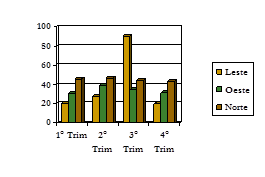
\includegraphics[width=6cm,height=4cm,keepaspectratio]{images/image1.png}
    }
    \label{fig:figura1}
    \fonte{xxxxxx}
\end{figure}


Se  buscada em alguma obra publicada, deve aparecer a fonte da figura, como no exemplo. Caso elaborada pelo próprio autor, incluir "Fonte: autor". Observando que na LISTA DE TABELAS a fonte não deve aparecer. 



\section{Descrição das Tabelas}

Veja exemplo de formatação da Tabela \ref{tab:tabela2}: a legenda aparece acima da tabela, a descrição deve ser centralizada, no número de identificação 2.1, o número 2 corresponde ao capítulo onde se localiza a tabela e o número 1 a ordem da tabela dentro do capítulo, seguido de dois ponto, espaço e  breve descrição, que deve ter a {\bf primeira} letra em maiúsculo. 

Assim como figuras, tabelas também devem indicar sua fonte. Caso elaboradas pelo próprio autor, incluir "Fonte: autor". Observando que na LISTA DE TABELAS a fonte não deve aparecer. 

Atente que {\bf as laterais das tabelas são abertas}. Isso torna a imagem mais limpa e clara. As tabelas do texto não devem exceder a margem.


\begin{table}[ht]
  \caption{Exemplo de apresentação de uma tabela no texto}
  \centering
    \begin{tabular}{ c | c | c }
        \hline 
        \textit{Manga} & 
        \textit{Abacaxi} &  
        \textit{Morango}  \\
        \hline
        12    & 100.000,00     & 10.000,00 \\
        \hline
        12    & 10.000,00     & 100.000,00 \\
      \hline
    \end{tabular}
   \fonte{EREGALI, 2004. p. 356.}
  \label{tab:tabela2}
\end{table}



%%%%%%%%%%%%%%%%%%%%%%%%%%%%%%%%%%%%%%%%%%%%%%%%%%%%%%%%%%%%%%%%%%%%%%%%%%%%%%%%%%%%%
% Capítulo 3
%
\chapter{Sobre referências e citações}

A classe \emph{iiufrgs} faz uso do pacote \emph{abnTeX2} com algumas alterações
feitas por Sandro Rama Fiorini. Culpe ele se algo der errado. Agradeça a ele
pelo que der certo. As modificações dão uma camada de tinta NATBIB-style,
já que o abntex2 usa uns comandos de citação feitos para alienígenas de 5 braços (wtf!?). \\

Exemplos de citação:
\begin{itemize}[leftmargin=3em]

\setlength{\itemindent}{1em}

 \item \textbf{cite}: Unicórnios são verdes \cite{Adams2009Conceptual};
    
 \item \textbf{citet}: Segundo \citet{Adams2009Conceptual}, unicórnios são verdes.
    
 \item \textbf{citeauthoronline e citeyearpar}: Segundo artigos de \citeauthoronline{Adams2009Conceptual}, unicórnios são verdes \citeyearpar{Adams2009Conceptual}.
    
\end{itemize}
 
 
 
Recomenda-se o uso de bibtex para gerenciar as referências (veja o arquivo
biblio.bib).



\section{citações}

Há duas formas de se fazer uma citação: a {\bf indireta} ou {\bf livre} (também chamada de {\it paráfrase}) e a {\bf citação direta} ou {\bf textual}. Pode haver, ainda, a {\bf citação de citação}.

Todas as citações devem trazer a {\bf identificação }de sua autoria.


\section{Citação Indireta ou Livre (paráfrase)}

Chamamos de citação indireta ou livre ({\it paráfrase}) aquela citação na qual expressamos o {\bf pensamento de outra pessoa }com {\bf nossas próprias palavras.}

Após fazermos a citação, devemos indicar o nome do autor, {\bf em letras minúsculas, }se estiver no corpo do texto, e com letras {\bf maiúsculas, }se estiver dentro dos parênteses, juntamente com o {\bf ano }da publicação da obra em que se encontra a idéia por nós referida. Não são indicadas páginas já que a idéia pode estar sendo resumida de uma obra inteira, de um capítulo, de diversas partes ou de um conjunto delas.

Desta forma (com o nome no corpo do texto):

Depois de analisar a situação, Nóvoa (1993) chegou a afirmar que o brasileiro ainda não está capacitado para escolher seus governantes por causa de sua precária vocação política e da absoluta falta de escolaridade, já que o homem do povo, o zé-povinho, geralmente não sabe sequer em quem votou nas últimas eleições, não sabe sequer quem são seus governantes, não saber sequer quem determina seu próprio meio de sobreviver.

Ou, então, (com o nome nos parênteses):

Depois de analisar a situação, chegou-se a afirmar que o brasileiro ainda não está capacitado para escolher seus governantes por causa de sua precária vocação política e da absoluta falta de escolaridade, já que o homem do povo, o zé-povinho, geralmente não sabe sequer em quem votou nas últimas eleições, não sabe sequer quem são seus governantes, não saber sequer quem determina seu próprio meio de sobreviver (NÓVOA, 1993).

No caso de o autor possuir outras obras, elas serão diferenciadas pela data da publicação. Havendo mais de uma obra no mesmo ano, acrescentamos uma letra após a data.

No caso do teatro ou do cinema quem melhor se definiu foi Antunes (1997-a) quando declarou que aqueles espaços haviam sido todos tomados pela geração de 40. Por outro lado, ele próprio se contradisse, mais tarde, (1997-b), como já se contradissera noutras ocasiões, ao referir-se às decisões tomadas pelos autores da geração de 50. Isso é uma incongruência com a qual convivemos há muito tempo.

Quando, no transcorrer do texto, em citações indiretas ou livres, se faz menção, seguidas vezes, ao mesmo autor, na mesma obra, {\bf {\it não é necessário}}{\it  }que{\it  }se repita a indicação do ano.


\begin{table}[ht]
  \caption{Deve-se escolher somente um tipo de citação para usar durante o texto}
  \centering
    \begin{tabular}{ l | p{8cm} }
        \hline
        \multicolumn{2}{c}{FORMATAÇÃO DAS CITAÇÕES DOS AUTORES DURANTE O TEXTO} \\
        \hline
        Nóvoa (1993) & O nome do autor deve ser escrito em letras {\bf minúsculas }quando apresentado no próprio texto \\
        \hline
        (GUIMARÃES, 1985, p.32) & O nome do autor deve ser escrito em letras {\bf maiúsculas }quando apresentado dentro dos parênteses. \\
      \hline
    \end{tabular}
  \\Fonte: MEREGALI, 2004. p. 356.
  \label{tab:tabela3}
\end{table}



\section{Citação Direta ou Textual (transcrição)}

São chamadas de citações diretas ou textuais aquelas em que se transcrevem {\bf exatamente as palavras do autor citado}. As citações diretas ou textuais podem ser {\bf breves }ou {\bf longas.}

São consideradas {\bf breves} aquelas cuja extensão não ultrapassa {\it três linhas. }Essas citações devem {\it integrar o texto e }devem vir {\bf entre aspas. O tamanho }da {\bf fonte }(letra) da citação breve {\bf permanece }o mesmo do corpo do texto {\bf {\it (12 pt).}}

Vimos que, para nosso esclarecimento, precisamos seguir os preceitos encontrados, já que Guimarães estabelece: "A valorização da palavra pela palavra encarna o objetivo precípuo do texto literário" (1985, p. 32) e, se isso não ficar bem esclarecido, nosso trabalho será seriamente prejudicado.

Ou assim:

Vimos que, para nosso esclarecimento, precisamos seguir os preceitos encontrados, já que ficou estabelecido que "a valorização da palavra pela palavra encarna o objetivo precípuo do texto literário" (GUIMARÃES, 1985, p.32) e, se isso não ficar bem esclarecido, nosso trabalho será seriamente prejudicado.

As citações com mais de três linhas são chamadas de {\bf longas }e devem receber um destaque especial{\bf  }com recuo (reentrada) de {\bf 4cm }ou {\bf dezesseis toques}, da margem, mais {\bf cinco }toques para o início do parágrafo, além de usar fonte 10 pt, justificada.

As citações longas, por já terem o destaque do recuo (reentrada), {\bf \underbar{não deverão ter aspas}} e o tamanho da fonte (letra) deve ser {\bf menor }que o do texto: {\bf {\it 10 pt.}}

A distância entre as linhas do corpo da citação deve ser de um espaço {\bf simples}. Entre o texto da citação e o restante do trabalho, deve-se deixar {\bf dois {\it espaços duplos, }}antes e depois.

Há uma certa dificuldade quanto ao reconhecimento de {\bf O}, {\bf A, OS, AS }como pronomes demonstrativos, mas essa dúvida é muito bem dirimida por Fernandes:

\begin{citacao}
Os pronomes O, A, OS e AS passam a ser pronomes demonstrativos sempre que numa frase puderem ser substituídos, sem alterar a estrutura dessa frase, respectivamente, por ISTO, ISSO, AQUILO, AQUELE, AQUELES, AQUELA, AQUELAS (1994, p. 19.).
\end{citacao}


Havendo {\bf supressão }de trechos {\bf dentro do texto }citado, faz-se a indicação com reticências entre colchetes {\bf [...]}: "Na comunicação diária, aquela comunicação que utilizamos no dia-a-dia, junto de nossos familiares e amigos, por exemplo, além da referencialidade da linguagem {\bf [...]} há pinceladas de função conativa" (CHALHUB , 1991, p. 37).

No {\bf início }ou no {\bf fim }da citação, as reticências são usadas apenas quando o trecho citado {\bf não é uma sentença completa}. Entende-se por sentença completa aquela que o autor elaborou, com todos os seus elementos, isto é, uma sentença que contenha sujeito, predicado e seus complementos gramaticais exigidos. Caso contrário, {\bf se a sentença for completa, }no início ou no termino de citação, {\bf não se deve fazer }o uso das reticências. {\bf É {\it óbvio}} que se trata de parte de um todo, que se retirou um trecho, portanto, não há necessidade de se indicar com as reticências.

Encerrava seu discurso nomeando os que figurariam somente nos exercício gerais, citando palavras de ordem, dentre as quais pudemos entender:

``... muitas mortes, desaparecimentos e desolação haverão de varrer este pais de norte a sul, de lesta a oeste e nada restará para a posteridade que sentirá a falta de um elo'' (MORGADO, 1967).

Mais adiante, aquilo que mais chocou a todos quanto o ouviam:

``Arrasem com tudo, queimem tudo, ponham tudo abaixo, destruam com tudo, não poupem ninguém, nem crianças, nem mulheres, nem velhos...'' (MORGADO, 1967).

Se a citação for usada para completar uma{\bf  }sentença do autor do Trabalho, esta terminará em vírgula e aquela iniciará {\bf sem a entrada de parágrafo} e com {\bf letra minúscula}. 

A secretária ameaçou, dizendo que, ``da próxima vez, a máquina ficará sem as peças de reposição, se ele não chegar e disser o que precisa ser dito, uma vez que não estou aqui para servir de adivinha para seus caprichos desencontrados e sem nexo.'' (MARQUES, 1982, p. 34).

Caso o texto do autor do Trabalho seja uma {\bf continuação }da citação, esta {\bf terminará por vírgula }e o texto reiniciado {\bf sem entrada de parágrafo e com letra minúscula.}

 Os gramáticos são claros quando assumem uma posição quanto ao emprego do pronome oblíquo no início de oração. Cegalla (l 991, p. 419) diz claramente que:

\begin{citacao}
 Iniciar a frase com o pronome átono só é lícito na conversação familiar, despreocupada, ou na língua escrita, quando se deseja reproduzir a fala dos personagens, porém nós sabemos que na prática não é bem assim que acontece - as normas, rigorosamente, são esquecidas por quase todos os usuários do idioma falado, principalmente nas ocasiões informais.
\end{citacao}

Quando houver uma citação {\bf {\it dentro de outra citação, }}as aspas da segunda transformam-se em aspas simples ( ' ) (apóstrofo${}^{: }$Não confundir a palavra {\bf {\it apóstrofo}}{\it  que }é o sinal (`), com {\bf {\it apóstrofe}}{\it  que }é uma figura de linguagem que consiste na interpelação ou invocação do leitor, ouvinte ou outra pessoa no decorrer de um texto). Quando dentro da citação transcrita houver aspas, estas também são mudadas para aspas simples.



Se for feita alguma {\bf interpelação, acréscimo }ou {\bf comentário }durante a citação, deve-se fazê-lo {\it entre colchetes }{\bf [ ]:}

Também chamado de corpo do trabalho, [o desenvolvimento] tem por finalidade expor, demonstrar e fundamentar a explicitação do assunto a ser abordado. É normalmente dividido em seções ou capítulos, que variam de acordo com a natureza do assunto. (GARCIA, 2000, p. 17.).

Se algum {\bf destaque }(grifo, negrito, itálico ou sublinhado) for dado, deve-se indicá-lo com a expressão {\bf grifo nosso, }entre colchetes:

A primeira citação de uma obra deve ter sua referência bibliográfica completa. As subseqüentes citações da mesma obra {\bf podem ser referendadas de forma abreviada, }desde que não haja referências intercaladas de outras obras do mesmo autor (NBR 6023-2000) {\bf [grifo nosso].} 

Caso o texto citado traga algum tipo de destaque dado pelo autor do trecho, devemos usar a expressão {\bf grifo do autor, entre colchetes.}

A verdadeira felicidade é encontrada nos pequenos detalhes que vão se somando {\bf dia após dia }de convivência com o ser amado (GUERRERO, 2000, p. 12) {\bf [grifo do autor].}

Quando o texto citado for composto por informações orais obtidas em aulas, palestras, debates, comunicações, etc. deve-se, entre parênteses, colocar a observação {\bf {\it informação oral, }}mencionando-se os dados disponíveis em nota de rodapé:

Eichenberg constatou que, na costa do Rio Grande do Sul, especialmente no litoral norte, há a presença abundante de conformes fecais, especialmente nos meses do verão (informação oral). Essa presença tem causado graves transtornos a todos os veranistas.

Se for o caso de se fazer menção a algo contido em {\it polígrafos, apostilas }ou quaisquer materiais avulsos, faz-se a indicação do nome do autor, quando for possível sua identificação, acrescentando-se a observação {\it `polígrafo', }`{\it material de propaganda', `panfleto', etc. }Procede-se da mesma forma com relação à data. Indica-se, se houver, caso contrário, registra-se s.d. (sem data). 



\section{Citação de Citação}

Se, num Trabalho, for feita uma citação de alguma passagem {\it já}{\bf {\it  }}{\it citada} em {\it outra obra, }a autoria deve ser referenciada pelo {\bf sobrenome do autor original }seguido da palavra latina {\bf apud }(que significa {\it segundo, conforme, de acordo com) }{\bf e o sobrenome do autor da obra consultada. }Dessa última, faz-se a referência completa (NBR6O23).

``O sistema consiste em colocar o recém-nascido no berço, ao lado da mãe, logo após o parto ou algumas horas depois, durante a estada de ambos na maternidade'' (HARUNARI apud GUARAGNA, 1992, p. 79).

Temos aí palavras de Harunari que foram citadas por Guaranga e que estão sendo utilizadas, agora, no meu trabalho.

{\bf Fonte:} FURASTÉ, Pedro Augusto. Normas Técnicas para o Trabalho Científico: explicitação das normas da ABNT. Porto Alegre: [s.n.], 2002. p. 49-56.

\noindent 


%%%%%%%%%%%%%%%%%%%%%%%%%%%%%%%%%%%%%%%%%%%%%%%%%%%%%%%%%%%%%%%%%%%%%%%%%%%%%%%%%%%%%
% Conclusões
%
\chapter{CONCLUSÃO}

Apresentar conclusão do trabalho...




%%%%%%%%%%%%%%%%%%%%%%%%%%%%%%%%%%%%%%%%%%%%%%%%%%%%%%%%%%%%%%%%%%%%%%%%%%%%%%%%%%%
% Referências 
%%%%%%%%%%%%%%%%%%%%%%%%%%%%%%%%%%%%%%%%%%%%%%%%%%%%%%%%%%%%%%%%%%%%%%%%%%%%%%%%%%%
%

%\bibliographystyle{abnt}

\bibliographystyle{abntex2-alf}


\bibliography{biblio} % arquivo que contém as referências (no formato bib). Colocar as suas lá (se tiver dúvida sobre como adicionar novas referências, usar o software JabRef ou Medley)



\noindent {\\\bf Se tiver alguma dúvida, veja os exemplos seguintes:}\\

\noindent {\bf \underbar{Monografia no todo}}\\

\noindent {\bf Livros e Anais de Congresso (Autor. Título. Edição. Local de Publicação: editora, ano de publicação).}\\

\noindent FURASTÉ, Pedro Augusto. {\bf Normas Técnicas para o Trabalho Científico}: explicitação das normas da ABNT. Porto Alegre: [s.n.], 2002. p. 49-56.

\noindent BRADLEY, N. {\bf The XML Companion}. 3${}^{rd}$ ed. Boston: Addison-Wesley, 2002.

\noindent FIELDS, D. K.; KDLB, M. A. {\bf Desenvolvendo na Web com JavaServer Pages}. Rio de Janeiro: Ciência Moderna, 2000.

\noindent OLIVEIRA, R. S. de; CARISSIMI, A. da S.; TOSCANI, S. S. {\bf Sistemas Operacionais}. 2.ed. Porto Alegre: Instituto de Informática da UFRGS: Sagra Luzzatto, 2001. 247 p. (Série Livros Didáticos, n.11).

\noindent SIMPÓSIO BRASILEIRO DE SISTEMAS MULTIMÍDIA E HIPERMÍDIA, SBMÍDIA, 7., 2001, Florianópolis. ... Florianópolis: UFSC: SBC, 2001.

\noindent NATIONAL CONFERENCE ON ARTIFICIAL INTELLIGENCE, AAII, 17., 2000. {\bf Proceedings}... Menlo Park, CA: AAAI Press: The MIT Press, 2000.

\noindent ~

\noindent {\bf \underbar{Parte de Monografia}}\\

\noindent {\bf Capítulo (Autor do capítulo. Título do capítulo. In: Autor/Editor/Organizador do livro. Título do livro. Edição. Local de publicação: editora, ano de publicação).}

\noindent LUBASZEWSKI, M.; COTA, E. F.; KRUG, M. R. Teste e Projeto Visando o Teste de Circuitos e Sistemas Integrados. In: REIS, R. A. da L. (Ed.) {\bf Concepção de Circuitos Integrados}. 2.ed. Porto Alegre: Instituto de Informática da UFRGS: Sagra Luzzatto, 2002. p. 167-189.

\noindent ROESLER, V.; BRUNO, G. G.; LIMA, J. V. de. ALM: Adaptative Layering Multicast. In: SIMPÓSIO BRASILEIRO DE SISTEMAS MULTIMÍDIA, SBMÍDIA, 7., 2001, Florianópolis. {\bf Anais...} Florianópolis: UFSC: SBC, 2001. p. 107-121.

\noindent PFEFFER, A.; KOLLER, D. Semantics and Inference for Recursive Probability Models. In: NATIONAL CONFERENCE ON ARTIFICIAL INTELLIGENCE, AAII, 17., 2000. {\bf Proceedings... }Menlo Park, CA: AAAI Press: The MIT Press, 2000.

\noindent ~

\noindent {\bf \underbar{Dissertações, teses, trabalhos individuais, etc.}}\\

\noindent MENEGHETTI, E. A. {\bf Uma Proposta de Uso da Arquitetura Trace como um Sistema de Detecção de Intrusão}. 2002. 105 f. Dissertação ( Mestrado em Ciência da Computação ) -- Instituto de Informática, UFRGS, Porto Alegre.

\noindent SABADIN, R. da S. {\bf QoS em Serviços de Suporte por Frame Relay}. 2000. 35 f. Trabalho Individual ( Mestrado em Ciência da Computação ) -- Instituto de Informática, UFRGS, Porto Alegre.

\noindent OTERO, I. M. {\bf Desenvolvimento de Sistema Cliente-Servidor em Camadas Utilizando Software Livre}. 2003. 55 f. Projeto de Diplomação ( Bacharelado em Ciência da Computação ) -- Instituto de Informática, UFRGS, Porto Alegre.

\noindent ~

\noindent {\bf \underbar{Artigo de periódico}}\\

\noindent GONÇALVES, L. M. G.; CESAR JUNIOR, R. M. Robótica, Sistemas Sensorial e Motos: principais tendências e direções. {\bf Revista de Informática Teórica e Aplicada}, Porto Alegre, v.9, n.2, p. 7-36, out. 2002.

\noindent JANOWIAK, R. M. Computers and Communications: a symbiotic relationship. {\bf Computer}, New York, v.36, n.1, p. 76-79, Jan. 2003.

\noindent ~

\noindent {\bf \underbar{Em meio eletrônico}}\\

\noindent LISBOA FILHO, J.; IOCHPE, C.; BORGES, K. Reutilização de Esquemas de Bancos de Dados em Aplicações de Gestão Urbana. {\bf IP -- Informática Pública}, Belo Horizonte, v.4, n.1, p.105-119, June 2002. Disponível em: $<$http://www.ip.pbh.gov.br/ip0401.html $>$. Acesso em: set. 2002.

\noindent ~

\noindent {\bf \underbar{RFC}}\\

\noindent CALLAGHAN, B.; PAWLOWSKI, B.; STAUBACH, P. {\bf NFS Version 3 Protocol Specification}: RFC 1831. [S.l.]: Internet Engineering Task Force, Network Working Group, 1995.

\noindent ~

\noindent {\bf \underbar{Norma}}\\

\noindent INSTITUTE OF ELECTRICAL AND ELECTRONIC ENGINEERING. {\bf IEEE 1003.1c-1995}: information technology -- portable operating system interface (POSIX), threads extension [C language]. New York, 1995.

\noindent ~

\noindent {\bf \underbar{Observações}}\\

Quando existirem mais de três autores, indica-se apenas o primeiro, acrescentando-se a expressão et al. Ex.: URANI, A. et al. Em casos em que a menção dos nomes for indispensável para certificar a autoria é facultado indicar todos os nomes.

Em caso de autoria desconhecida, a entrada é feita pelo título. Ex.: DIAGNÓSTICO do Setor Editorial Brasileiro. São Paulo: Câmara Brasileira do Livro, 1993.

Quando houver uma indicação de edição, esta deve ser transcrita, utilizando-se abreviaturas dos numerais ordinais e da palavra edição, ambas na forma adotada na língua do documento.

Ex.: SCHAM, D. {\bf Schawm's Outline of Theory and Problems}. 5${}^{th}$ ed. New York: Schawm Publishing, 1956.

PEDROSA, I. {\bf Da Cor a Cor Inexistente}. 6. ed. Rio de Janeiro: L. Cristiano, 1995.

Não sendo possível determinar o local (cidade) de publicação, utiliza-se à expressão sine loco, abreviada, entre colchetes [S.l.].

Quando a editora não puder ser indicada, deve-se indicar a expressão sine nomine, abreviada, entre colchetes [s.n].

Quando o local e a editora não puderem ser identificados, utilizam-se [S.l.:s.n].


\end{comment}

\end{document}
